\documentclass[11pt]{amsart}


\usepackage{geometry}                % See geometry.pdf to learn the layout options. There are lots.
\geometry{a4paper}                   % ... or a4paper or a5paper or ...
%\geometry{landscape}                % Activate for for rotated page geometry
\usepackage[parfill]{parskip}    % Activate to begin paragraphs with an empty line rather than an indent
\usepackage{enumitem}
\usepackage{graphicx}
\usepackage{amssymb}
\usepackage{amsmath}
\usepackage{cancel}
\usepackage{tikz}
\usepackage{epstopdf}
\DeclareGraphicsRule{.tif}{png}{.png}{`convert #1 `dirname #1`/`basename #1 .tif`.png}
\usepackage{breqn}

\usetikzlibrary{calc,intersections,through,backgrounds,arrows,decorations.markings}

\tikzset{
  coordsys/.pic={
    \draw[->] (0,0) -- ++(6mm,0pt);
    \draw[->] (0,0) -- ++(0pt,6mm);
  },
  myarr/.style={decoration={
      markings,
      mark=between positions 0 and 1 step 2mm with {\arrow{stealth}},
    },
    postaction=decorate
  },
}

\title{Econ 210C Problem Set \# 3}
\author{Nathaniel Bechhofer}
%\date{}                                           % Activate to display a given date or no date

\begin{document}
\maketitle


\section{Variable labor supply in the RBC model}
\begin{figure}[h]
	\centering
	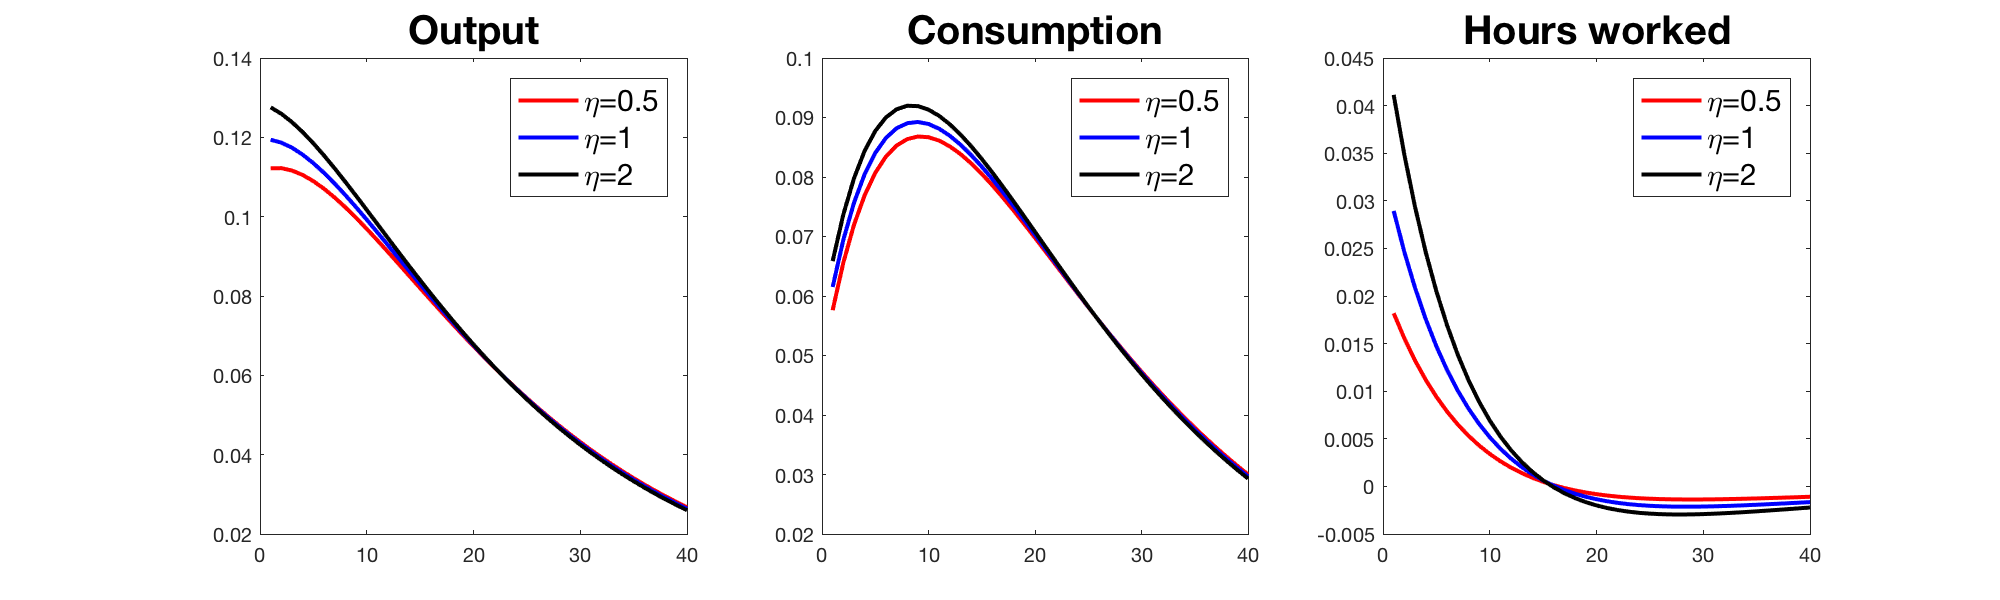
\includegraphics[width=\textwidth]{Minki/Q1}
	\caption{Impulse responses with varying $\eta$}
\end{figure}

\begin{table}[h]
	\centering
	\begin{tabular}{ccccc}
		\hline \hline 
		& $\eta=0.5$  & $\eta = 1$          & $\eta = 2$ & Data  \\
		\hline 
		$\sigma_Y$ &  1.54    & 1.64    & 1.74    & 1.72     \\
		$\sigma_C$ &  0.97    & 1.02   & 1.08       & 1.27 \\
		$\sigma_L$ &   0.23   &  0.37   & 0.53     &  1.59 \\
		\hline
	\end{tabular}
	\caption{Response to a transitory discount factor shock}
\end{table}
Larger Frisch elasticity values imply a better fit, as they generate stronger inter-temporal substitution of labor supply, amplifying the effect of shocks. 
Consumption is still too smooth, and the volatility of hours is too low. 

\newpage

\section{Variable capital utilization in an RBC model}

\subsection*{(a)}

Firms choose capital utilization $U$, capital $K$, and labor demand $N$.

The production function that we can use directly (since the output is the numeraire) is
\[
Y_t = (U_t K_{t-1})^{\alpha} (Z_t N_t)^{1-\alpha}
\]
and since the firms own capital, they face the constraint
\[
K_t = I_t + (1 - \delta(U_t)) K_{t-1}
\]
but they also have to pay wages $W_t N_t$ and invest $I_t$
so we can set up the Lagrangian
\begin{tiny}
\[
\mathcal{L} = E \sum_s (\prod_{k=1}^s (1+r_{t+k})^{-1}) \bigg{(} (U_{t+s} K_{t+s-1})^{\alpha} (Z_{t+s} N_{t+s})^{1-\alpha} - W_{t+s} N_{t+s} - I_{t+s} + q_{t+s} (-K_{t+s} +  I_{t+s} + (1 - \delta(U_{t+s})) K_{t+s-1}) \bigg{)}
\]
\end{tiny}
so we have first order conditions:

for labor we have
\[
W_t = (1-\alpha) (U_{t} K_{t-1})^{\alpha} Z_{t}^{1-\alpha} N_t^{-\alpha}
\]
for investment we have
\[
q_t = 1
\]
for capital at time $t$ we have
\[
q_t = E \left[ \frac{1}{1+r_{t+1}} \left( \alpha U_{t+1}^{\alpha} K_t^{\alpha -1} (Z_{t+1} N_{t+1})^{1-\alpha} + q_{t+1} (1 - \delta(U_{t+1}))  \right) \right]
\]
and finally we have the condition for utilization
\[
\alpha U_t^{\alpha - 1} K_{t-1}^{\alpha} (Z_{t} N_{t})^{1-\alpha} = q_t K_{t-1} \delta'(U_t)
\]

Combining the investment and capital optimality conditions yields the expression for the rental rate of capital. 
\[
	R_{t+1} = \alpha U_{t+1}^{\alpha} K_t^{\alpha -1} \left(Z_{t+1} N_{t+1}  \right)^{1-\alpha} - \delta(U_{t+1})
\]
The rental rate depends on utilization because the marginal product of capital and its depreciation rate depend on utilization. 

\subsection*{(b)}
The log linearized version of the utilization optimality condition
	 \[
	 q_t \delta^{'}(U_t) K_{t-1}  = \alpha U_t^{\alpha -1} K_{t-1}^\alpha \left( Z_t N_t \right)^{1-\alpha}
	 \] 
	 is
	\begin{align*}
	&\check{q_t}+ \frac{\delta^{''}(\bar{U}) \bar{U}}{\delta^{'}(\bar{U})} \check{U}_t + \check{K}_{t-1} = (\alpha -1) \check{U_t} + \alpha \check{K_{t-1}}  + (1-\alpha) \left(  \check{Z_t} + \check{N_t}\right) 
	\end{align*}
We know $\check{q_t}=0$ from the investment optimality condition and  we also know 
\[
\check{Y_t} = \alpha \left( \check{U_t} + \check{K_{t-1}} \right) + (1-\alpha) \left(  \check{Z_t} + \check{N_t}\right)
\] 
because the production function is given, so we have
	\begin{align*}
	\check{U_t} = \frac{1}{1 + \Delta} \left( \check{Y_t} - \check{K_{t-1}}\right)
	\end{align*}

\subsection*{(c)}

The log-linearized production function is
	\begin{align*}
	\check{Y_t} &= \alpha \left( \check{U_t} + \check{K_{t-1}} \right) + (1-\alpha) \left(  \check{Z_t} + \check{N_t}\right) \\
	& = \frac{\alpha}{1 + \Delta} \left( \check{Y_t} - \check{K_{t-1}} \right) + \alpha \check{K_{t-1}} + (1-\alpha ) \left(  \check{Z_t} + \check{N_t}\right)
	\end{align*} 
	Isolate $\check{Y_t}$:
	\begin{align*}
	\check{Y_t} &= \frac{\Delta \alpha }{1 + \Delta - \alpha} \check{K_{t-1}} + \frac{(1+\Delta)(1-\alpha)}{1+ \Delta - \alpha} \left(  \check{Z_t} + \check{N_t} \right)  \\
	& = \check{Z_t} + \check{N_t} \quad \left( \text{when } \Delta = 0 \right) \\
	& = \alpha \check{K_{t-1}} + (1-\alpha) \left( \check{Z_t } + \check{N_t} \right)   \quad \left( \text{when } \Delta = \infty \right)
	\end{align*}

     $\Delta = 0$ implies the capital stock is impotent, and output thus only depends on technology and labor. 
$\Delta = \infty$ implies full utilization, so output depends on all three inputs, with weights equal to the Cobb-Douglas coefficients. 
    
In every other case, we have 
    \begin{equation*}
    \check{Y_t} = \frac{\Delta \alpha }{1 + \Delta - \alpha} \check{K_{t-1}} + (1-\alpha) \left( \check{Z_t} + \check{N_t} \right)+ \frac{\alpha (1-\alpha)}{1+ \Delta - \alpha} \left(  \check{Z_t} + \check{N_t} \right)
    \end{equation*}
    so $Z_t$ and $N_t$ in $Y_t$ matter relatively more (with capital not being fully utilized) relative to the $\Delta = \infty$ case. 

\subsection*{(d)} 

The labor supply curve is: 
    \begin{equation*}
    L_t = W_t^{\frac{1}{\chi}}
    \end{equation*}
    and thus $\chi >0$ assumption does not allow indeterminacy.
    
The linearized labor demand function is $\check W_t = \check Y_t - \check N_t$, so we have
\[
 \check W_t =  \frac{\Delta \alpha }{1 + \Delta - \alpha} \check{K_{t-1}} + \frac{(1+\Delta)(1-\alpha)}{1+ \Delta - \alpha} \left(  \check{Z_t} + \check{N_t} \right) - \check N_t 
 \]
 showing that labor demand is downward sloping.
    
If labor exhibits increasing returns to scale we can get indeterminacy, but
    \begin{align*}
    &\frac{(1+\Delta)(1-\alpha)}{1+ \Delta - \alpha} > 1  \\
    \rightarrow & \frac{-\Delta \alpha}{1 + \Delta - \alpha } > 0 
    \end{align*}
shows we require $1 + \Delta < \alpha$. 
With Cobb-Douglas production $0 < \alpha < 1$, indeterminacy is impossible in this model.  


\section{Homework in macroeconomics}

\subsection*{(a)}

 The Lagrangian for the household's maximization problem is:
\[
	\mathcal{L} = \left( C_m^\rho + C_h^\rho \right)^{\frac{1}{\rho}} - \left( \frac{1}{\eta} + 1 \right)^{-1} \left(  L_h + L_m \right)^{\frac{1}{\eta} + 1} + \lambda \left( W L_m - C_m \right) + \xi \left(L_h - C_h \right)
\]
	The first order conditions for the interior solutions are:
	\begin{align*}
	\cancel{\frac{1}{\rho}}\left( C_m^\rho + C_h^\rho \right)^{\frac{1}{\rho} -1} \cancel{\rho}  C_m^{\rho-1} &= \lambda \\
	\cancel{\frac{1}{\rho}} \left( C_m^\rho + C_h^\rho \right)^{\frac{1}{\rho} -1} \cancel{\rho} C_h^{\rho-1} & = \xi \\
	\left(  L_h + L_m \right)^{\frac{1}{\eta} }  &=\lambda W \\
	\left(  L_h + L_m \right)^{\frac{1}{\eta} }  &= \xi 	 
	\end{align*}

\subsection*{(b)}

From the two first order conditions for labor, we have 
\[
\xi = \lambda W
\]

\subsection*{(c)}

From the two first order conditions for consumption, we have
\[
\xi = \lambda \left( \frac{C_h}{C_m} \right)^{\rho-1}
\]

\subsection*{(d)}

With the budget constraints binding, we have
\[
C_h = L_h
\]
and from above we get
\[
C_h = C_m W^{\frac{1}{\rho-1}}
\]

\subsection*{(e)}

We now have
\[
L_h = C_m W^{\frac{1}{\rho-1}}
\]
and we can assume the budget constraint holds for formal markets to make the substitution
\[
C_m = WL_m
\]
getting us
\[
L_h = WL_m W^{\frac{1}{\rho-1}}
\]
equivalent to
\[
L_h = L_m W^{\frac{\rho}{\rho-1}}
\]
and from our first order conditions we have
\[
L_h + L_m = (\lambda W)^{\eta}
\]
so we can substitute for $L_h$ to get
\[
(\lambda W)^{\eta} - L_m = L_m W^{\frac{\rho}{\rho-1}}
\]
so we have
\[
L_m (1 + W^{\frac{\rho}{\rho-1}}) = (\lambda W)^{\eta}
\]
and thus
\[
L_m = \frac{(\lambda W)^{\eta}}{(1 + W^{\frac{\rho}{\rho-1}})}
\]

\subsection*{(f)}

We now have
\[
\frac{\partial L_h}{\partial W} = \frac{(1 + W^{\frac{\rho}{\rho-1}}) \lambda^{\eta} \eta W^{\eta - 1} - (\lambda W)^{\eta} (\frac{\rho}{\rho-1}) W^{\frac{\rho}{\rho-1} - 1}}{(1 + W^{\frac{\rho}{\rho-1}})^2}
\]
with 
\[
\frac{\partial L_m}{\partial W} \cdot \frac{W}{L_m} = \frac{(1 + W^{\frac{\rho}{\rho-1}}) \eta  -  (\frac{\rho}{\rho-1}) W^{\frac{\rho}{\rho-1}}}{(1 + W^{\frac{\rho}{\rho-1}})}
\]
as the elasticity of $L_h$ with respect to $W$.

\subsection*{(g)}

If home production can perfectly substitute for market production, then when wages are lower than the value of the home produced goods, labor will not be supplied to markets. 
As $\rho$ gets smaller, the Frisch elasticity approaches $\eta$. 
With no substitution, the Frisch elasticity equals $\eta$ exactly. 
	


\subsection*{(h)}

We had
\[
\left( C_m^\rho + C_h^\rho \right)^{\frac{1}{\rho} -1}  C_m^{\rho-1} = \lambda
\]
so substitute the budget constraints
\[
((W L_m)^{\rho} + L_h^{\rho})^{\frac{1}{\rho} -1} (W L_m)^{\rho-1} = \lambda
\]
and use the substitution
\[
L_h = L_m W^{\frac{\rho}{\rho-1}}
\]
to get
\[
((W L_m)^{\rho} + ( W^{\frac{\rho^2}{\rho-1}}) L_m^{\rho})^{\frac{1}{\rho} -1} (W L_m)^{\rho-1} = \lambda
\]
so now substitute back in to
\[
L_m = \frac{(\lambda W)^{\eta}}{(1 + W^{\frac{\rho}{\rho-1}})}
\]
and we have
\[
L_m = \frac{ \left[((W L_m)^{\rho} + ( W^{\frac{\rho^2}{\rho-1}}) L_m^{\rho})^{\frac{1}{\rho} -1} (W L_m)^{\rho-1}\right]^{\eta} W^{\eta}}{(1 + W^{\frac{\rho}{\rho-1}})}
\]
and we can simplify to get
\[
L_m = \frac{ \left[((W^{\rho} + W^{\frac{\rho^2}{\rho-1}}) L_m^{\rho})^{\frac{1}{\rho} -1} (W L_m)^{\rho-1}\right]^{\eta} W^{\eta}}{(1 + W^{\frac{\rho}{\rho-1}})}
\]
and again to get
\[
L_m = \frac{ \left[(W^{\rho} + W^{\frac{\rho^2}{\rho-1}})^{\frac{1}{\rho} -1} L_m^{1-\rho} (W L_m)^{\rho-1}\right]^{\eta} W^{\eta}}{(1 + W^{\frac{\rho}{\rho-1}})}
\]
and the $L_m$ terms on the right side cancel so we have
\[
L_m = \frac{ \left[(W^{\rho} + W^{\frac{\rho^2}{\rho-1}})^{\frac{1}{\rho} -1}  W ^{\rho-1}\right]^{\eta} W^{\eta}}{(1 + W^{\frac{\rho}{\rho-1}})}
\]
and we can rewrite the numerator to get
\[
L_m = \frac{ \left[(W^{\rho} + W^{\frac{\rho^2}{\rho-1}})^{\frac{1}{\rho} -1}  W ^{\rho}\right]^{\eta} }{(1 + W^{\frac{\rho}{\rho-1}})}
\] 
equivalent to 
\[
L_m = \frac{ \left[(W^{\rho}(1 + W^{\frac{\rho}{\rho-1}}))^{\frac{1}{\rho} -1}  W ^{\rho}\right]^{\eta} }{(1 + W^{\frac{\rho}{\rho-1}})}
\] 
and
\[
L_m = \frac{ \left[(1 + W^{\frac{\rho}{\rho-1}})^{\frac{1}{\rho} -1}  W^{1-\rho} W ^{\rho}\right]^{\eta} }{(1 + W^{\frac{\rho}{\rho-1}})}
\] 
and
\[
L_m = \frac{ \left[(1 + W^{\frac{\rho}{\rho-1}})^{\frac{1}{\rho} -1}  W \right]^{\eta} }{(1 + W^{\frac{\rho}{\rho-1}})}
\] 
to finally get
\[
L_m = \left( 1 + W^{\frac{\rho}{\rho-1}} \right)^{\eta \left( \frac{1-\rho}{\rho} \right) -1} W^\eta
\]

\subsection*{(i)}

Differentiating, we have
\[
\frac{\partial L_m}{\partial W} = \frac{\rho  \left(\frac{\eta  (1-\rho )}{\rho }-1\right) W^{\eta +\frac{\rho }{\rho -1}-1} \left(W^{\frac{\rho }{\rho -1}}+1\right)^{\frac{\eta  (1-\rho )}{\rho }-2}}{\rho -1}+\eta  W^{\eta -1} \left(W^{\frac{\rho }{\rho -1}}+1\right)^{\frac{\eta  (1-\rho )}{\rho }-1}
\]
and we have the elasticity as
\[
\frac{\partial L_m}{\partial W} \cdot \frac{W}{ L_m} = \frac{\rho  \left(\frac{\eta  (1-\rho )}{\rho }-1\right) W^{\frac{\rho }{\rho -1}} \left(W^{\frac{\rho }{\rho -1}}+1\right)^{-1}}{\rho -1} + \eta 
\]
which simplifies to 
\[
\frac{\partial L_m}{\partial W} \cdot \frac{W}{ L_m} =  \eta +\frac{\rho  \left(\eta  \left(\frac{1}{\rho }-1\right)-1\right)}{(\rho -1) \left(W^{\frac{\rho }{1-\rho }}+1\right)}
\]

\subsection*{(j)}

Very low values of $\rho$, implying high elasticity between market and home consumption, can help deliver the high labor supply elasticity.




\section{$q$-Theory with Variable Capital Utilization}

\subsection*{(a)}

Firms choose utilization, investment, and labor to maximize the expected value of 
\[
\sum_{s} \left( \prod_{k=1}^{s} \left(1 + r_{t+k} \right) \right)^{-1} 
\times   Z_{t+s} \left( U_{t+s} K_{t+s-1}  \right)^{\alpha} L_{t+s}^{1-\alpha}  - W_{t+s} L_{t+s} - I_{t+s} \left[ 1 + \phi \left( \frac{I_{t+s}}{K_{t+s-1}} \right) \right] 
\]
given the constraints
\[
\left( -K_{t+s} + (1-\delta(U_t))K_{t+s-1} + I_{t+s} \right) = 0
\]
This problem is truly dynamic because the adjustment cost links the present and future period investment decisions. 

\subsection*{(b)}
The first order conditions are
\begin{align*}
		\frac{\partial \mathcal{L}}{\partial L_t}: &\quad  w_t = (1-\alpha) \frac{Y_t}{L_t} \\
		\frac{\partial \mathcal{L}}{\partial L_t}: & \quad q_t = 1 + \phi \bigg ( \frac{I_t}{K_t} \bigg ) + \frac{I_t}{K_t} \phi' \bigg ( \frac{I_t}{K_t} \bigg ) \\
		\frac{\partial \mathcal{L}}{\partial K_t}: & \quad q_t = (1+r_{t+1})^{-1} \bigg ( \alpha \frac{Y_{t+1}}{K_{t+1}} + \frac{I_{t+1}^2}{K_{t+1}^2} \phi' \bigg ( \frac{I_t}{K_t} \bigg ) + q_{t+1} (1-\delta(U_{t+1})) \bigg ) \\
		\frac{\partial \mathcal{L}}{\partial U_t}: &\quad  \alpha \frac{Y_t}{U_t} = q_t \delta'(U_t) K_t
	\end{align*}
	Combining the second and third equations, we can get an expression for the rental rate of capital: 
	\begin{equation*}
	r_{t+1} = \alpha \frac{Y_{t+1}}{K_{t+1}} + \frac{I_{t+1}^2}{K_{t+1}^2} \phi' \bigg ( \frac{I_t}{K_t} \bigg )  + \delta(U_{t+1})
	\end{equation*}
	The rental rate of capital is a function of utilization because the depreciation rate and the marginal product of capital depend on utilization. 
	It is also a function of $q$ because replacing capital is costly, so optimizing requires taking into account just how far the firm is from equalizing replacement cost and marginal value for capital.
	
	\subsection*{(c)}
	 The log-linearized version of the FOC for utilization is:
	\begin{align*}
	\check U_t = \frac{\check Y_t  - \check K_t - \check q_t}{1 + \Delta} = \frac{\check{MPK}_t - \check q_t}{1 + \Delta} \\
	\end{align*}
	Thus we have that the sign of the percentage deviation of utilization from its steady state value depends on the percentage change in $ MPK_t -  q_t$.  
	Here $q_t$ is the ratio of the value of additional unit of capital to its replacement cost, not always 1. 
	The percentage change in $ MPK_t -  q_t$ is the net gain of adding one more unit of capital in the production. When this is positive, it is profitable for the firm to use more capital, implying $\check U_t >0$. 
	
	\subsection*{(d)} 
	Utilization is negatively correlated with $q$. 
	Since $q$ and investment are positively correlated, procyclical investment can imply counter-cyclical utilization depending on the procyclicality of $MPK$. 
	
	\subsection*{(e)} When a technology shock looks approximately permanent, it is profitable to accumulate capital, meaning $\check{MPK} <0$. 
	$U_t$ is therefore countercyclical in the high persistence case. 
	Accumulating more capital necessitates reduced utilization to prevent depreciation. 
	
	$U_t$ can be procyclical when the shock is transitory, because the increased capital won't be worth much when the shock is over; $\check{MPK} >0$.
	



\section{Fiscal multiplier in the RBC model}

\subsection*{(a)}

		The log-linearized system of equations is
	\begin{align*}
		&\check{K}_t = (1-\delta) \check{K}_{t-1} + \delta \check{I}_t \\
		&\check{C}_t + \frac{1}{\eta} \check{L}_t = \check{Y}_t - \check{L}_t \\
		&E_t \check{C}_{t+1} - \check{C}_t = \frac{\alpha \frac{\bar{Y}}{\bar{K}}}{\alpha \frac{\bar{Y}}{\bar{K}} + (1-\delta)} (E_t \check{Y}_{t+1} - \check{K}_t ) \\
		&\check{Y}_t = \alpha \check{K}_{t-1} + (1-\alpha) \check{L}_t \\
		&\check{Y}_t = \frac{\bar{C}}{\bar{Y}} \check{C}_t + \frac{\bar{I}}{\bar{Y}} \check{I}_t + \frac{\bar{G}}{\bar{Y}} \check{G}_t \\
		&\check{G}_t = \rho_g \check{G}_{t-1} + \epsilon_t^g
	\end{align*}
	Guess that the policy functions take the form
	\begin{align*}
		&\check{C}_t = v_{CK} \check{K}_{t-1} + v_{CG} \check{G}_{t} \\
		&\check{K}_t = v_{KK} \check{K}_{t-1} + v_{KG} \check{G}_{t}
	\end{align*}
	Now plug the policy functions into the system of equations and we are left with the log-linearized consumption Euler equation and labor-leisure condition in terms of parameters, coefficients of the policy functions, and state variables:
	\begin{dmath*}
		(v_{CK} v_{KK} - v_{CK}) \check{K}_{t-1} + (v_{CK} v_{KG} + v_{CG}\rho_g - v_{CG}) \check{G}_{t} = \frac{\alpha \frac{\bar{Y}}{\bar{K}}}{\alpha \frac{\bar{Y}}{\bar{K}} + (1-\delta)} \left[ \frac{\bar{C}}{\bar{Y}} v_{CK} v_{KK} + \frac{\bar{I}}{\bar{Y}} (v_{KK} - 1 + \delta) v_{KK} \frac{1}{\delta} - v_{KK} \right] \check{K}_{t-1} + \frac{\alpha \frac{\bar{Y}}{\bar{K}}}{\alpha \frac{\bar{Y}}{\bar{K}} + (1-\delta)} \left[ \frac{\bar{C}}{\bar{Y}} v_{CK} v_{KG} + \frac{\bar{C}}{\bar{Y}} v_{CG} \rho_g + \frac{\bar{I}}{\bar{Y}} (v_{KK} - 1 + \delta) v_{KG} \frac{1}{\delta} + \frac{\bar{I}}{\bar{Y}} v_{KG} \rho_g \frac{1}{\delta} + \frac{\bar{G}}{\bar{Y}} \rho_g - v_{KG} \right] \check{G}_t
	\end{dmath*}
	\begin{dmath*}
		\left[ v_{CK} - \left( \frac{1}{\eta} + 1 \right) \frac{\alpha}{1-\alpha} \right] \check{K}_{t-1} + v_{CG} \check{G}_t = \frac{-\alpha - \frac{1}{\eta}}{1-\alpha} \left[ \frac{\bar{C}}{\bar{Y}} v_{CK} + \frac{\bar{I}}{\bar{Y}} (v_{KK} - 1 + \delta) \frac{1}{\delta} \right] \check{K}_{t-1} + \frac{-\alpha - \frac{1}{\eta}}{1-\alpha} \left[ \frac{\bar{C}}{\bar{Y}} v_{CG} + \frac{\bar{I}}{\bar{Y}} v_{KG} \frac{1}{\delta} + \frac{\bar{G}}{\bar{Y}} \right] \check{G}_{t}
	\end{dmath*}
	By comparing the coefficients on $\check{K}_{t-1}$ and $\check{G}_t$ in both equations, we obtain 4 equations
	\begin{dmath*}
		v_{CK} v_{KK} - v_{CK} = \frac{\alpha \frac{\bar{Y}}{\bar{K}}}{\alpha \frac{\bar{Y}}{\bar{K}} + (1-\delta)} \left[ \frac{\bar{C}}{\bar{Y}} v_{CK} v_{KK} + \frac{\bar{I}}{\bar{Y}} (v_{KK} - 1 + \delta) v_{KK} \frac{1}{\delta} - v_{KK} \right]
	\end{dmath*}
	\begin{dmath*}
		v_{CK} v_{KG} + v_{CG}\rho_g - v_{CG} = \frac{\alpha \frac{\bar{Y}}{\bar{K}}}{\alpha \frac{\bar{Y}}{\bar{K}} + (1-\delta)} \left[ \frac{\bar{C}}{\bar{Y}} v_{CK} v_{KG} + \frac{\bar{C}}{\bar{Y}} v_{CG} \rho_g + \frac{\bar{I}}{\bar{Y}} (v_{KK} - 1 + \delta) v_{KG} \frac{1}{\delta} + \frac{\bar{I}}{\bar{Y}} v_{KG} \rho_g \frac{1}{\delta} + \frac{\bar{G}}{\bar{Y}} \rho_g - v_{KG} \right]
	\end{dmath*}
	\begin{dmath*}
		v_{CK} - \left( \frac{1}{\eta} + 1 \right) \frac{\alpha}{1-\alpha} = \frac{-\alpha - \frac{1}{\eta}}{1-\alpha} \left[ \frac{\bar{C}}{\bar{Y}} v_{CK} + \frac{\bar{I}}{\bar{Y}} (v_{KK} - 1 + \delta) \frac{1}{\delta} \right]
	\end{dmath*}
	\begin{dmath*}
		v_{CG} \check{G}_t = \frac{-\alpha - \frac{1}{\eta}}{1-\alpha} \left[ \frac{\bar{C}}{\bar{Y}} v_{CG} + \frac{\bar{I}}{\bar{Y}} v_{KG} \frac{1}{\delta} + \frac{\bar{G}}{\bar{Y}} \right] \check{G}_{t}
	\end{dmath*}
	
	Solving numerically, we get
	\begin{align*}
	v_{CK} &\approx 0.66 \\
	v_{CG} &\approx -0.09 \\
	v_{KK} &\approx 0.97 \\
	v_{KG} &\approx -0.01 
	\end{align*}

\subsection*{(b)}
	
	The increase in government expenditure is only temporary, and the boost in output is transitory. Households compensate for the increased government expenditure by decreasing consumption, decreasing savings, and increasing labor supply. The households desired level of steady-state capital remains unchanged. This causes MPL (and wages) to decline while MPK (and interest rate) to increase.
	This is shown in Figure \ref{5b}.
	\begin{figure}[htbp]
\begin{center}
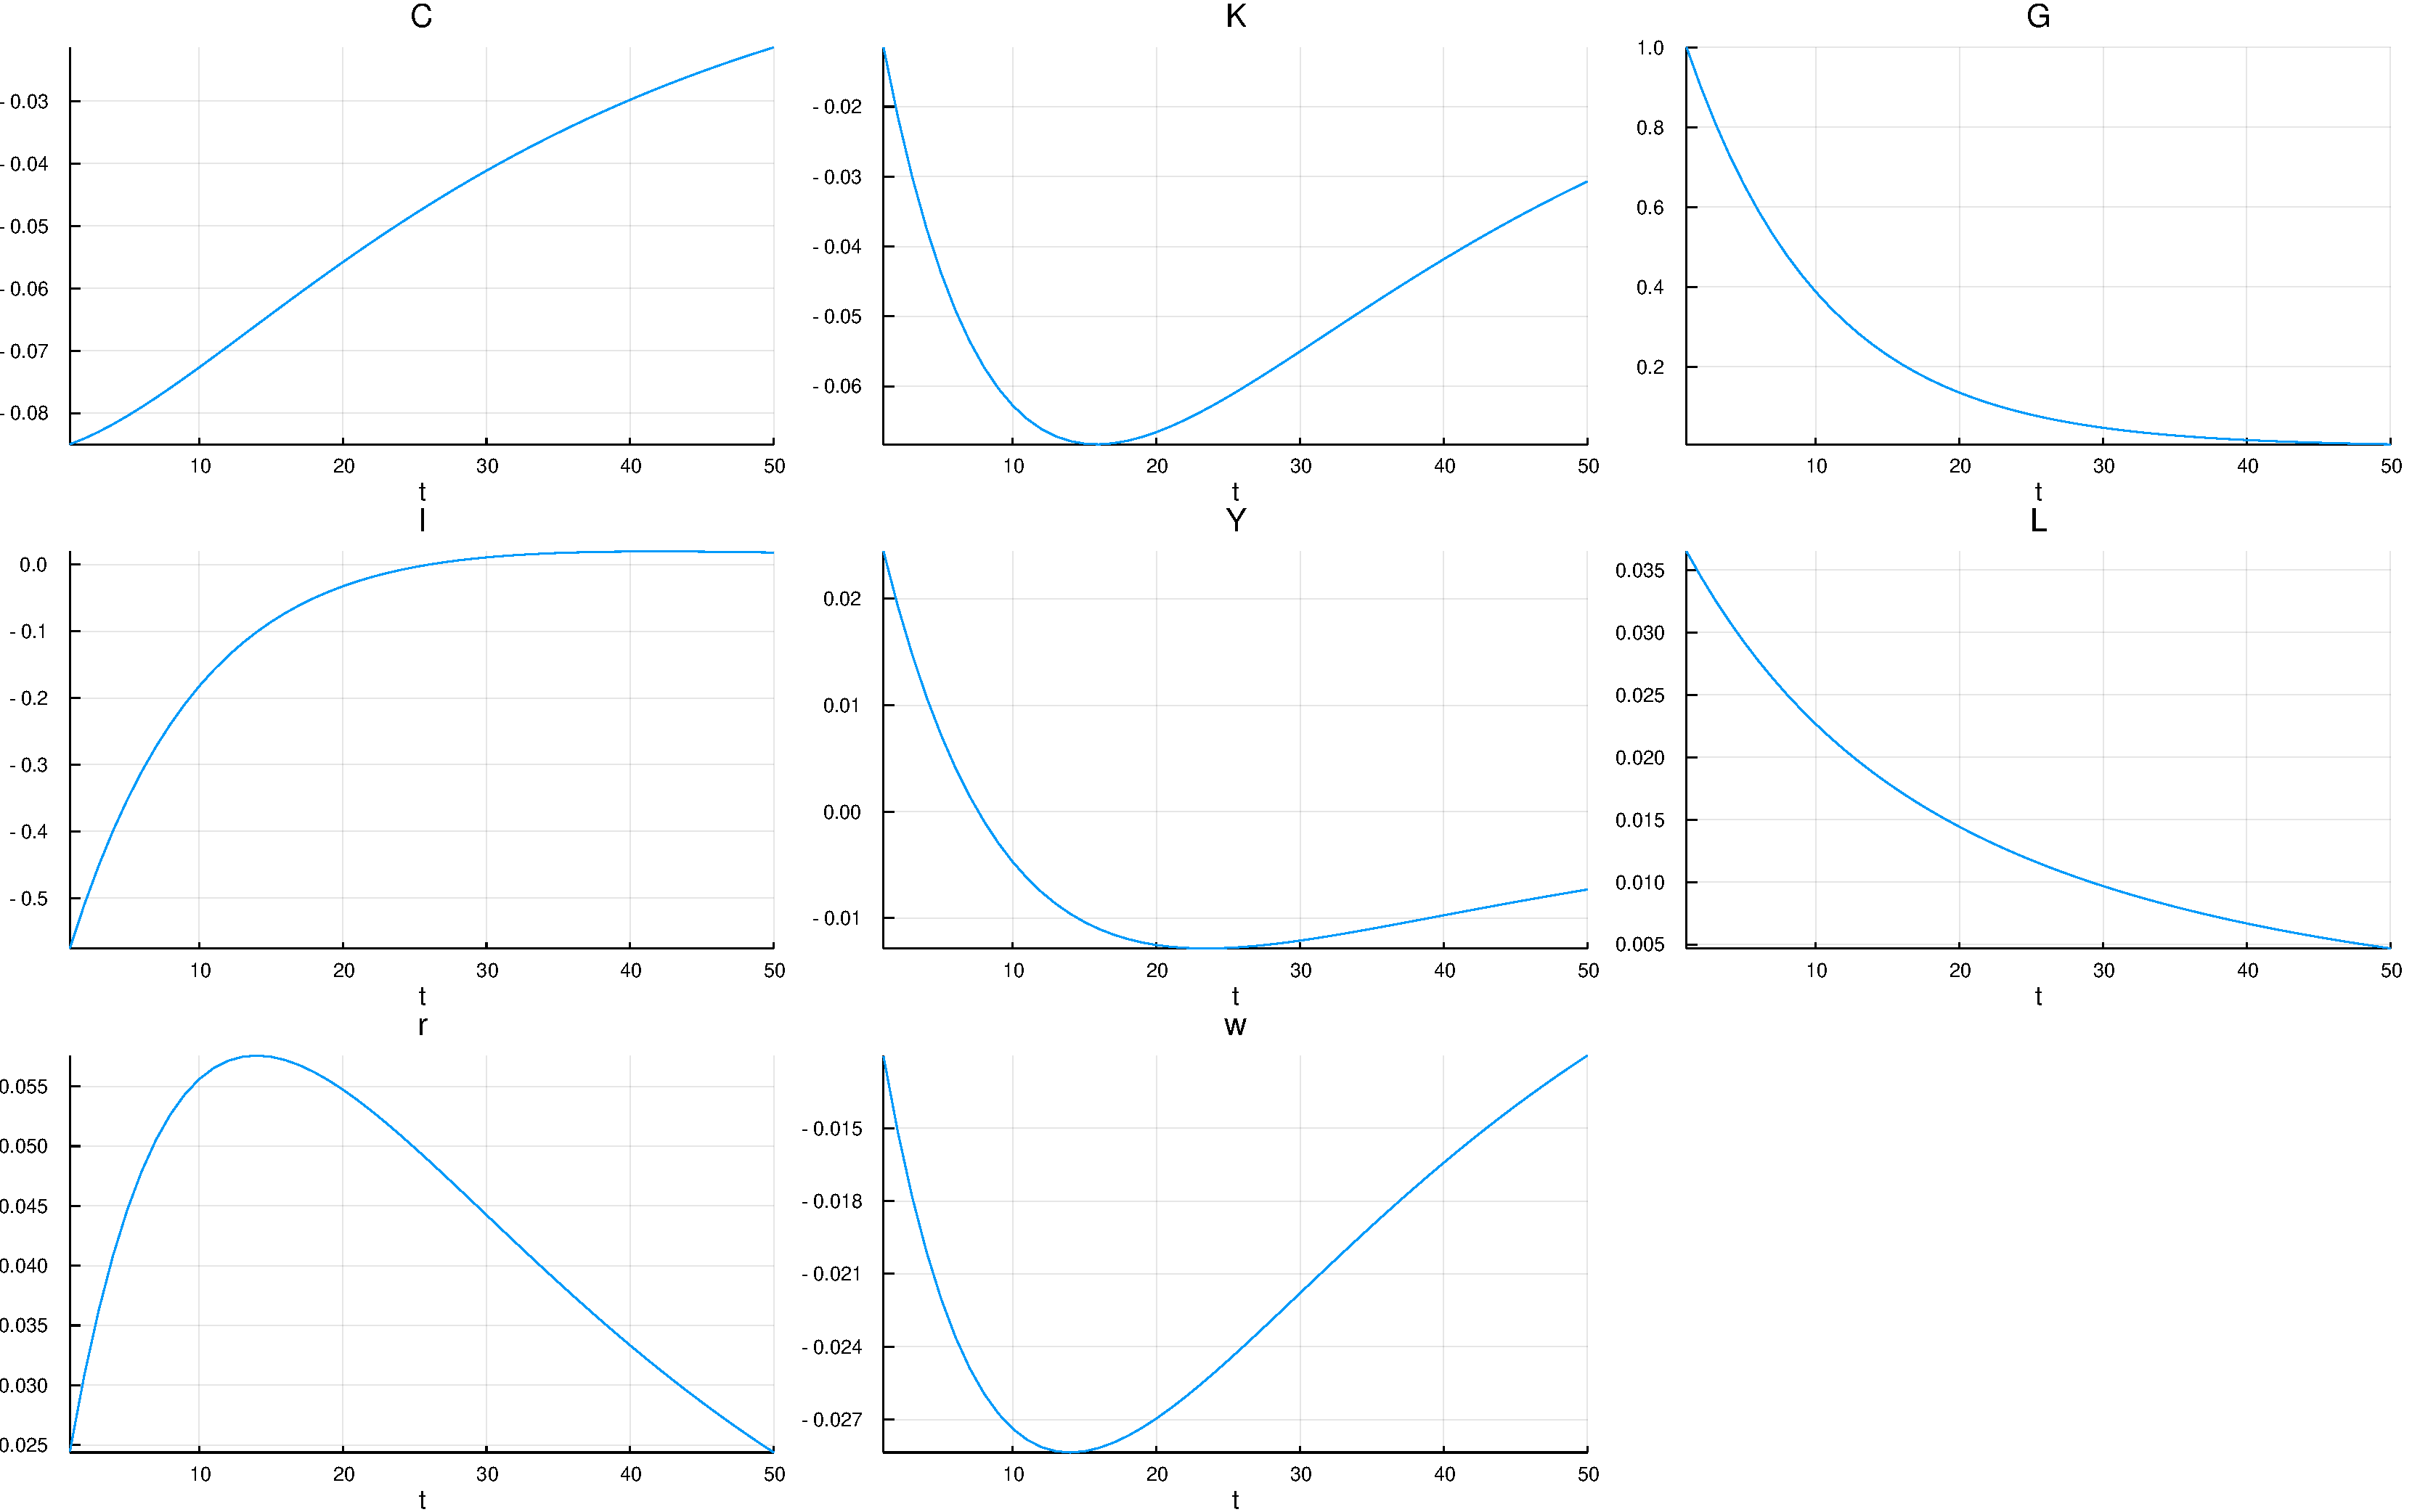
\includegraphics[width=\textwidth]{Ken/output/IRF_b_plot.pdf}
\caption{Impulse response to a unit shock in government spending.}
\label{5b}
\end{center}
\end{figure}


\subsection*{(c)}
	
	The multiplier is about 1.13. The new impulse response is shown in Figure \ref{5c}.
	\begin{figure}[htbp]
\begin{center}
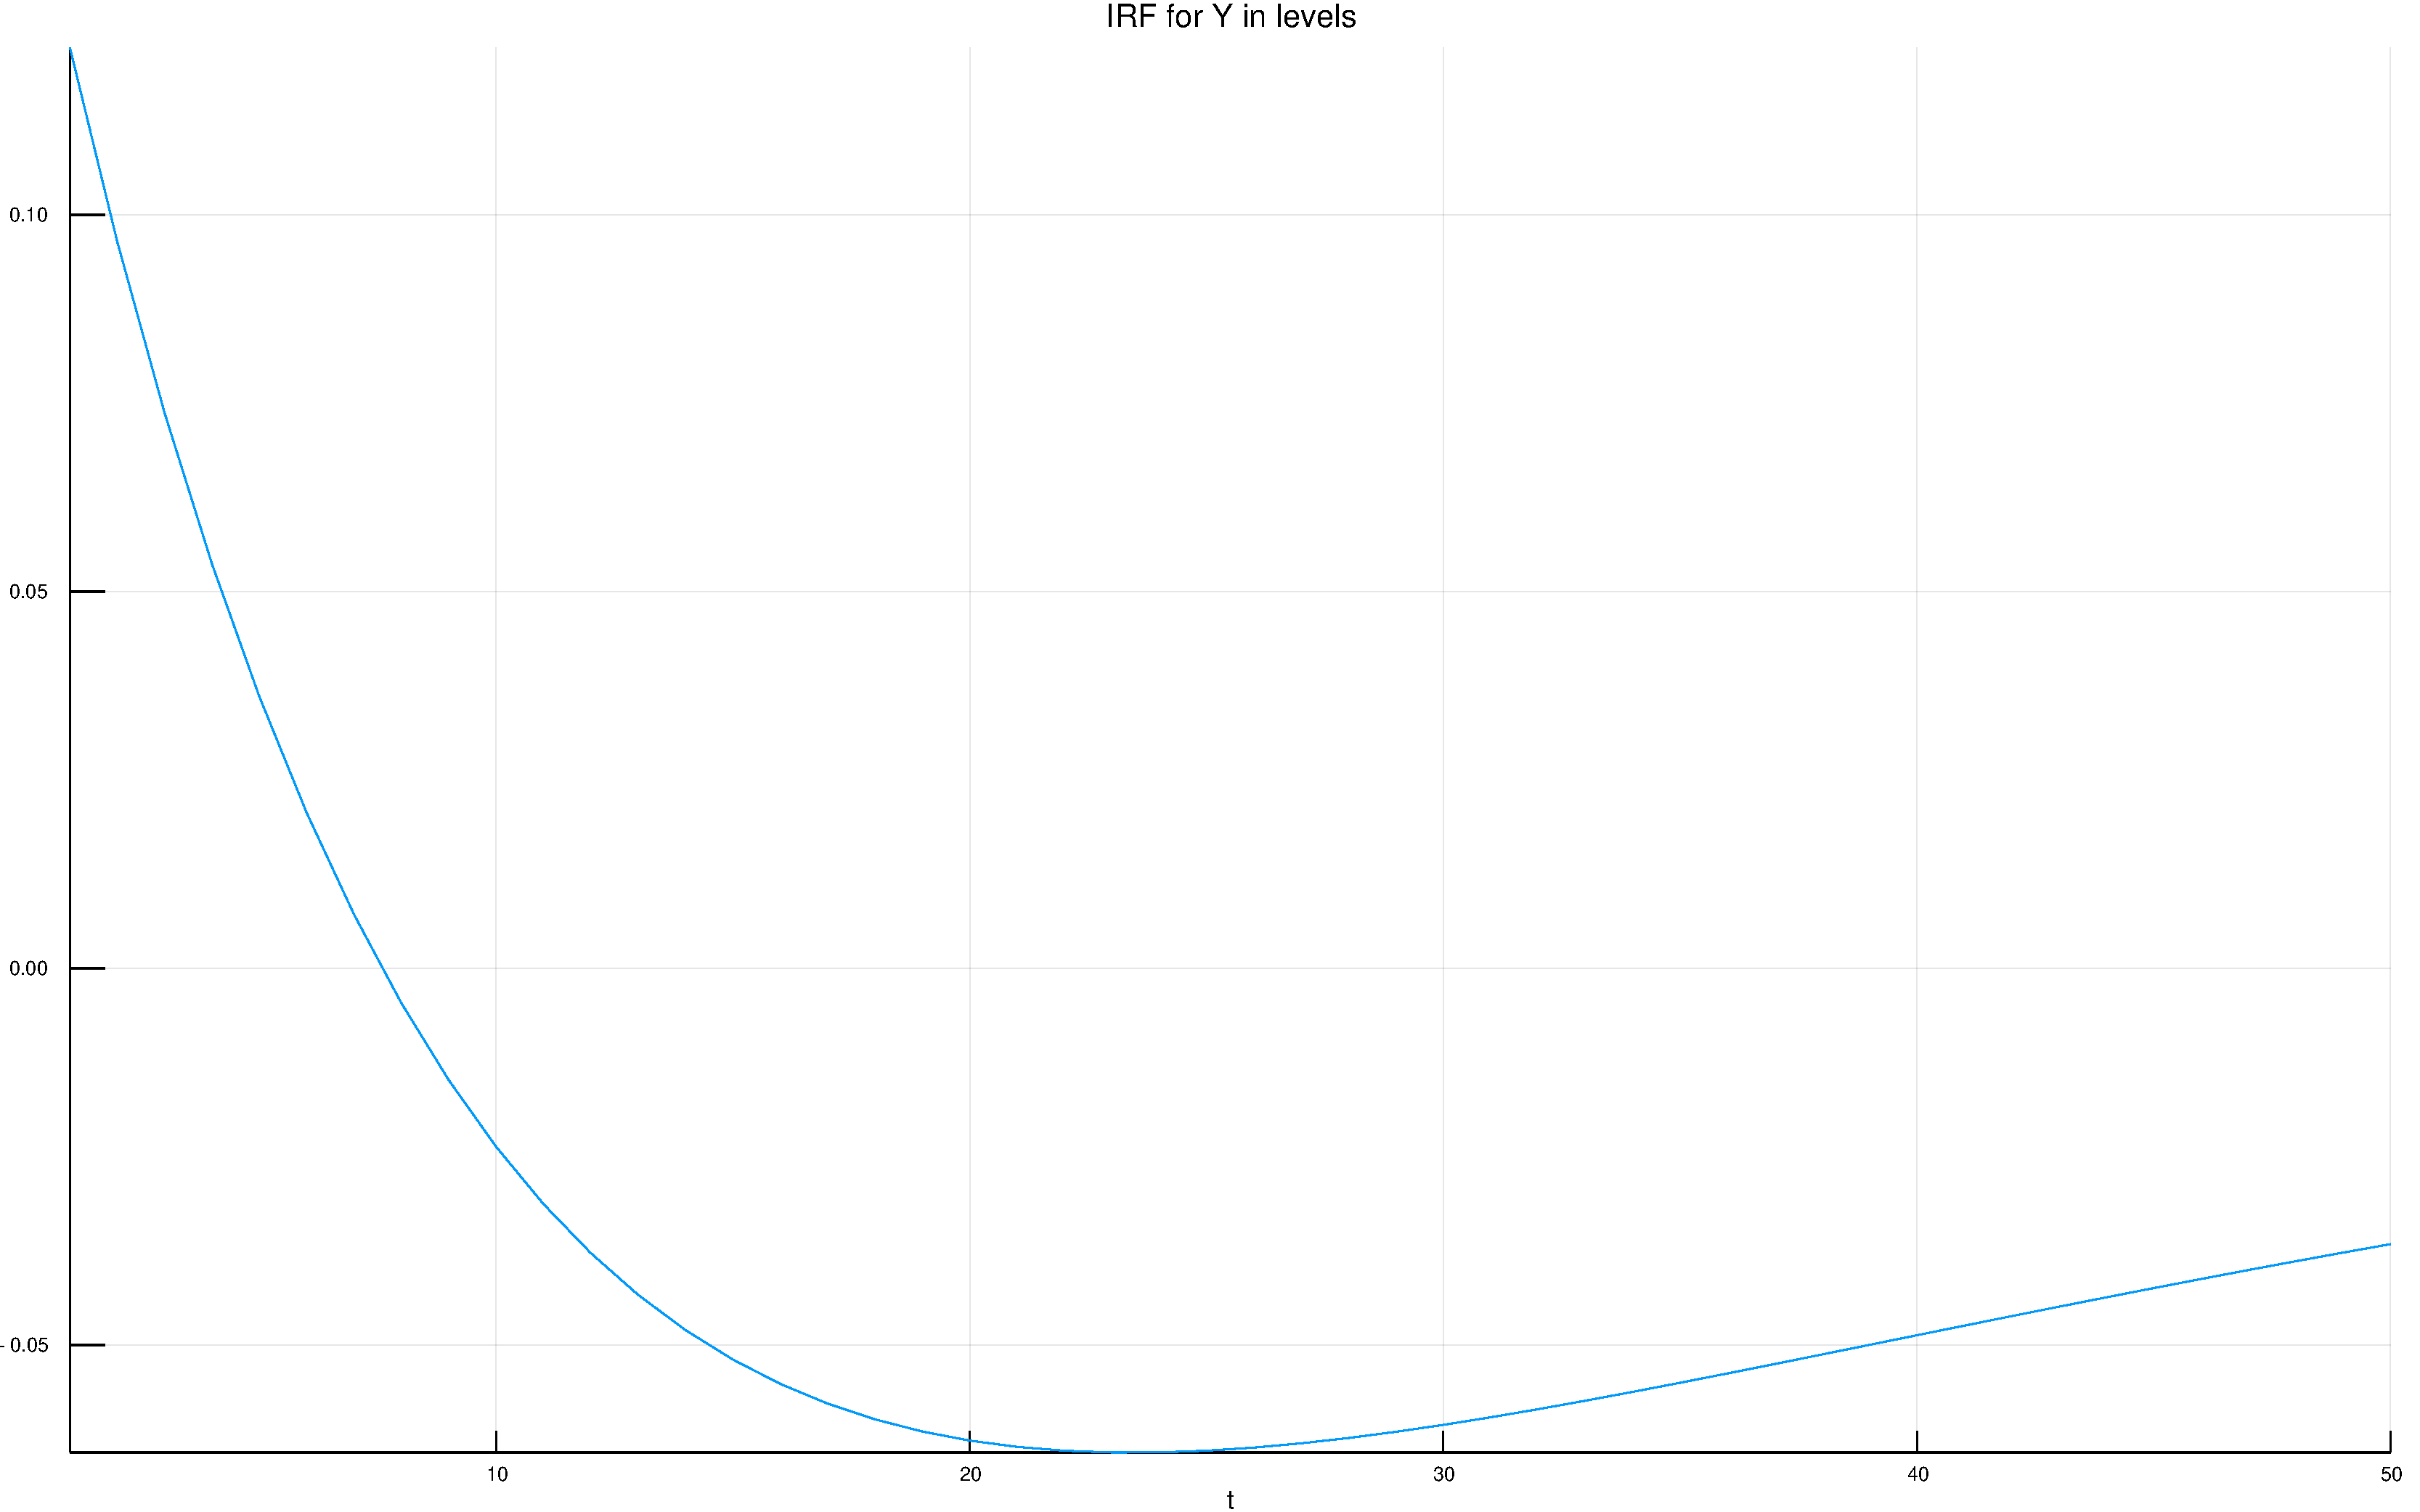
\includegraphics[width=\textwidth]{Ken/output/IRF_c_plot.pdf}
\caption{Impulse response to a unit shock in government spending in levels.}
\label{5c}
\end{center}
\end{figure}

\subsection*{(d)}

We now have
	\begin{align*}
	v_{CK} &\approx 0.66 \\
	v_{CG} &\approx -0.27 \\
	v_{KK} &\approx 0.97 \\
	v_{KG} &\approx 0.003 
	\end{align*}
	
	Increased output persists, so households decrease consumption and increase labor supply even more as a result of increased savings to get a higher level of steady-state capital. This increase in labor supply causes wages to decline by more and the interest rate to increase more. The level of increase in output is much larger; the multiplier is about 1.4.
	
	\begin{figure}[htbp]
\begin{center}
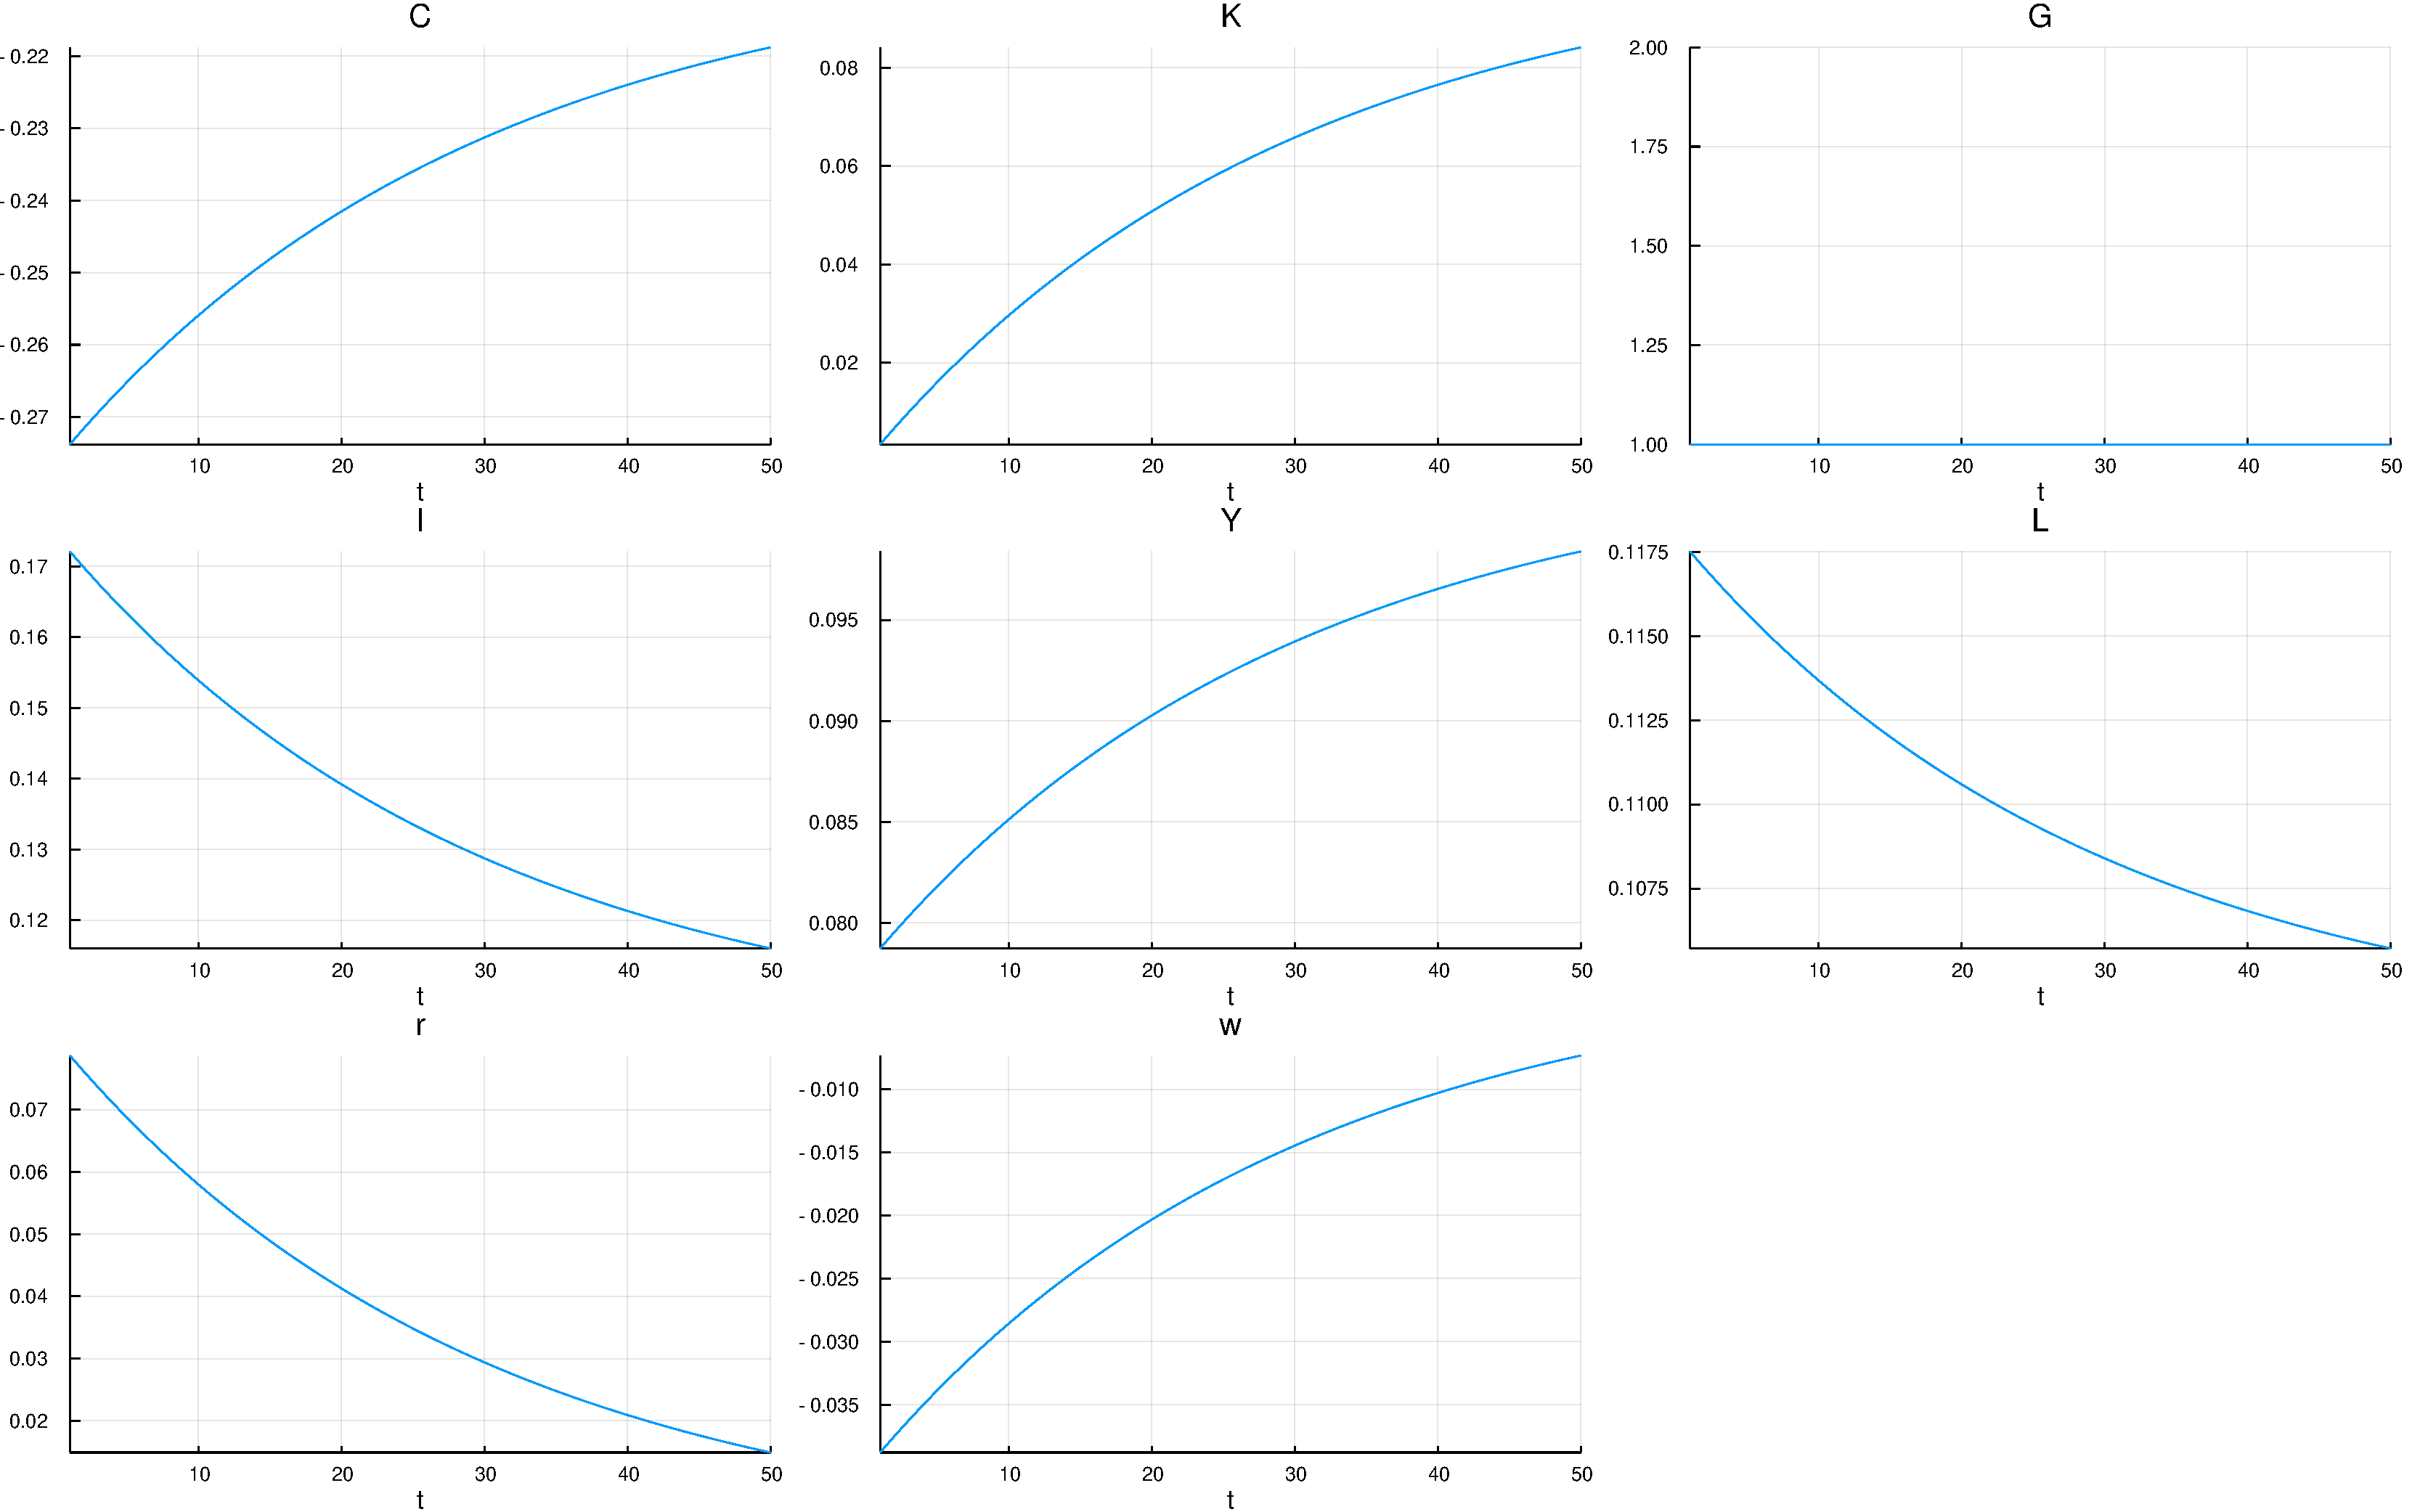
\includegraphics[width=\textwidth]{Ken/output/IRF_d_plot.pdf}
\caption{Impulse response to the permanent shock}
\label{5d}
\end{center}
\end{figure}


\begin{figure}[htbp]
\begin{center}
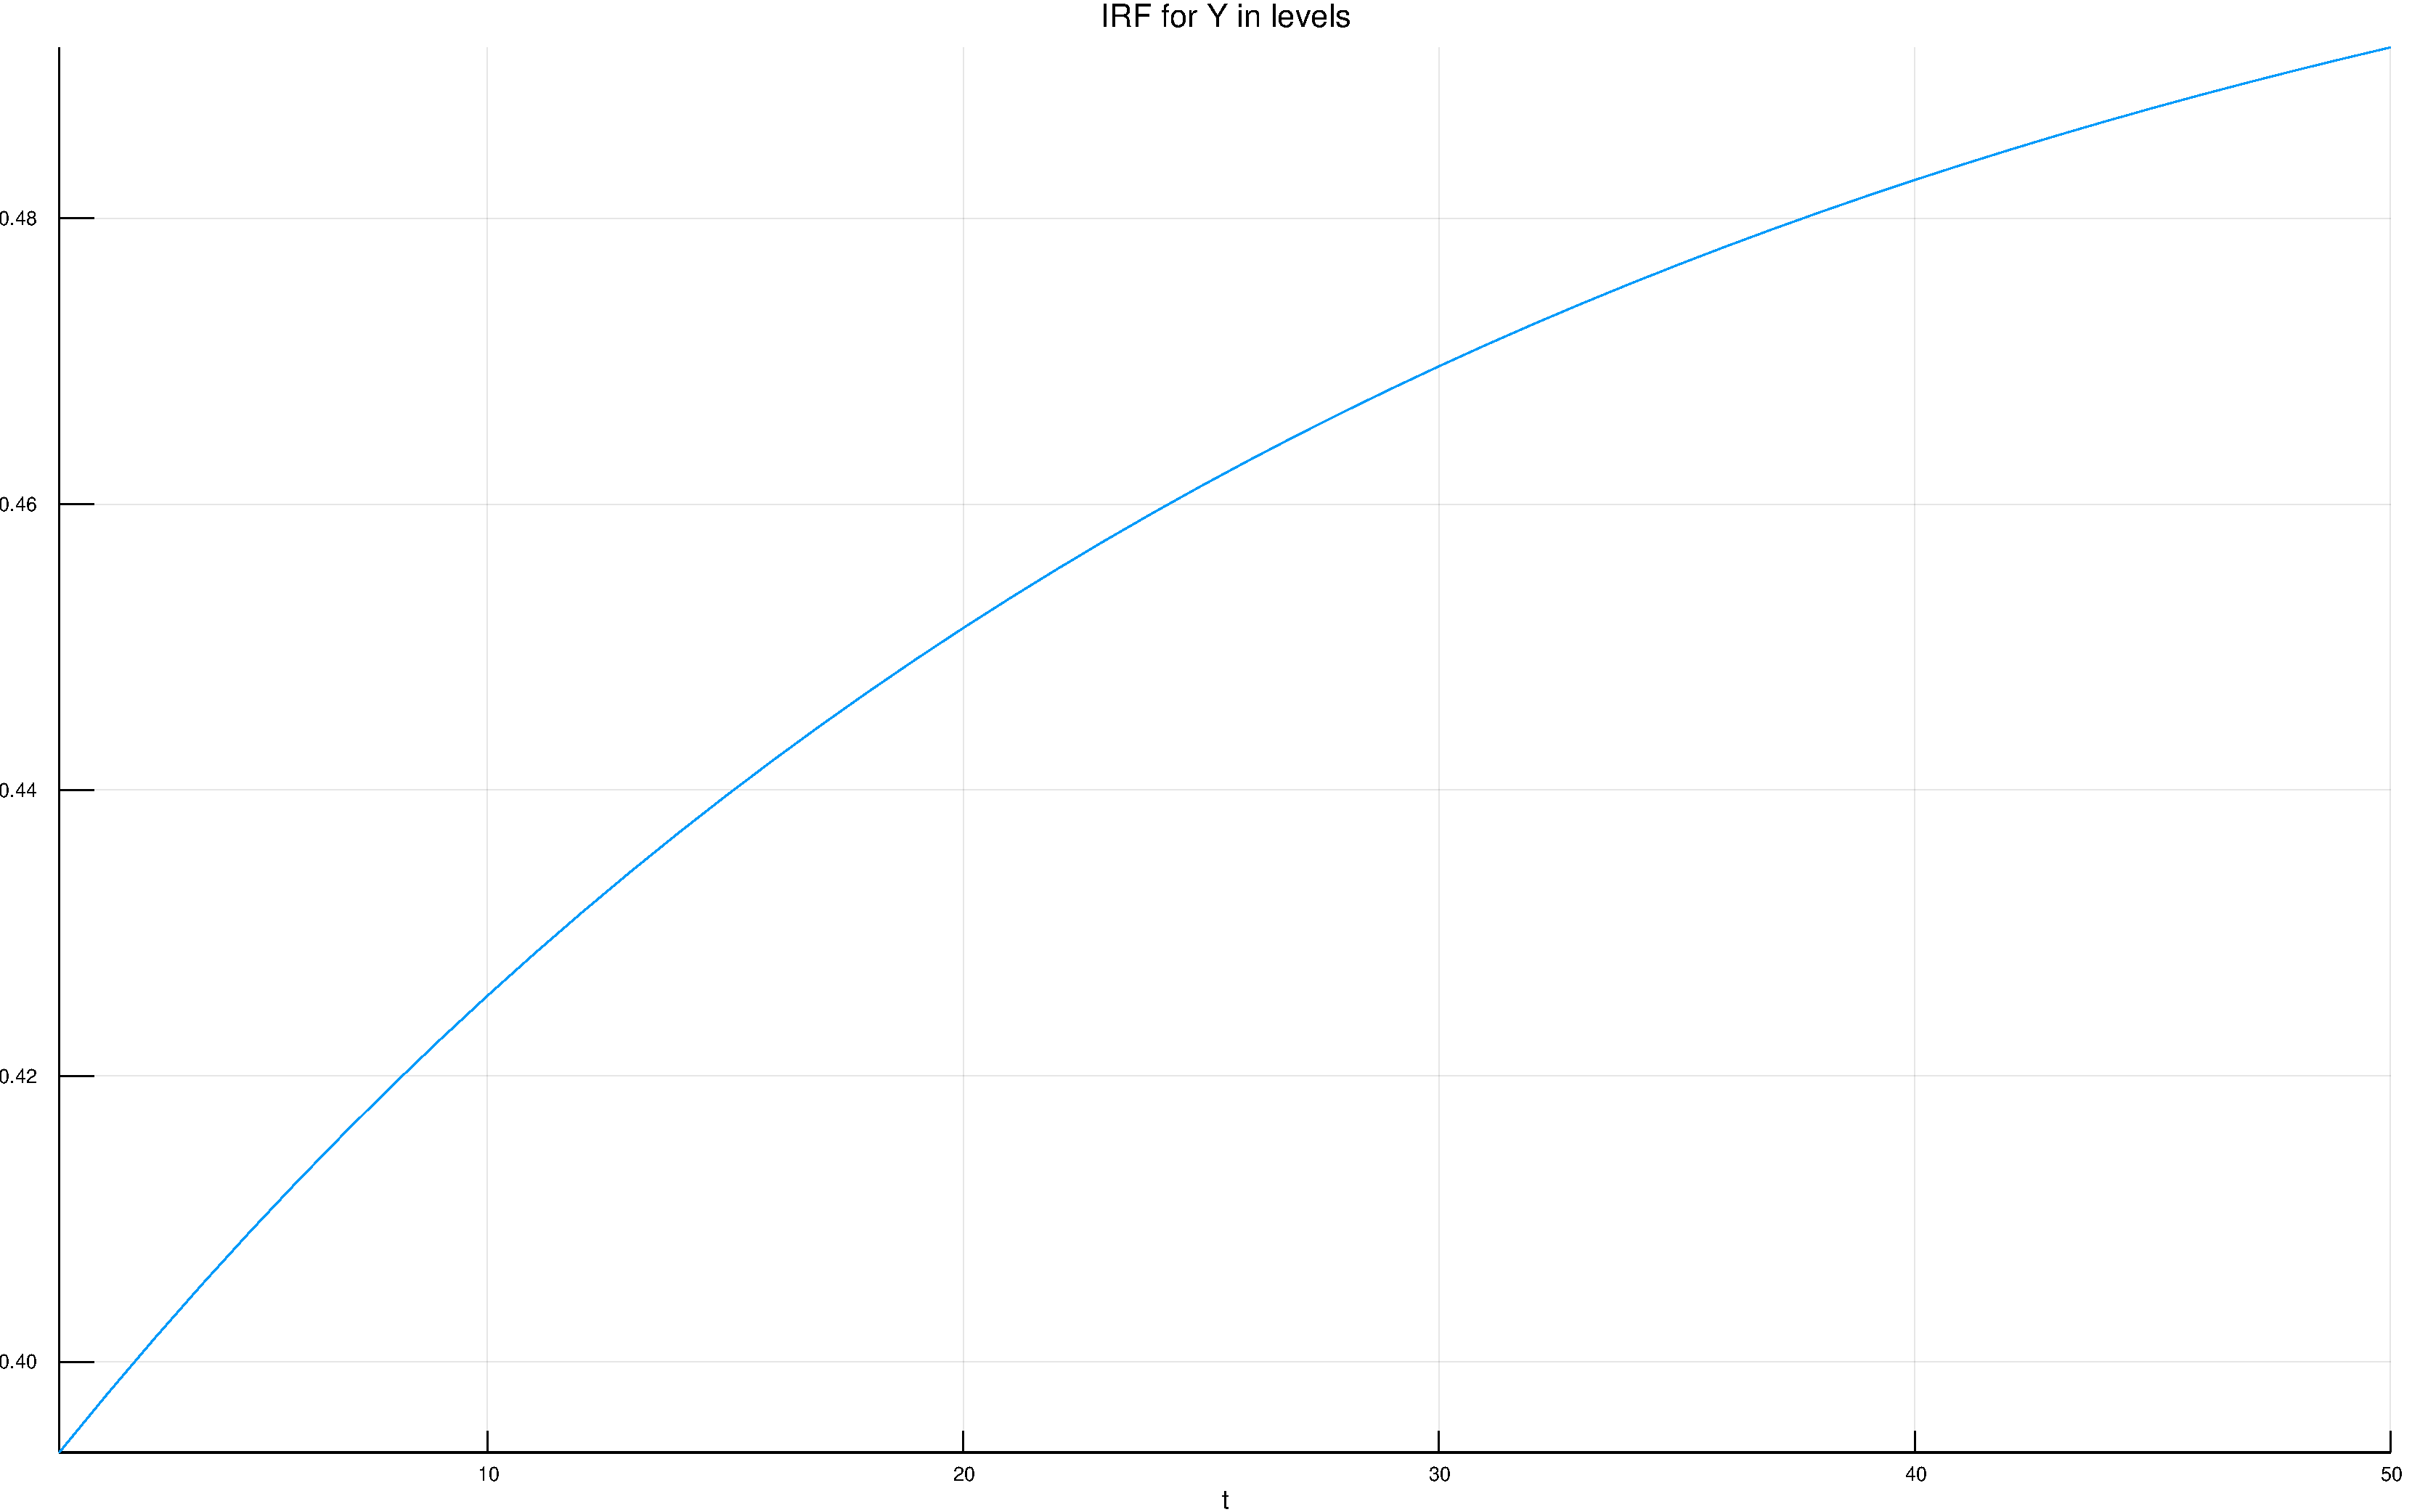
\includegraphics[width=\textwidth]{Ken/output/IRF_d_Y_plot.pdf}
\caption{Impulse response to the permanent shock in levels}
\label{5b}
\end{center}
\end{figure}



\end{document}